\documentclass[12pt,a4paper]{article}

% Margins.
\setlength{\oddsidemargin}{0in}
\setlength{\evensidemargin}{0in}
\setlength{\headheight}{12pt}
\setlength{\headsep}{42pt}
\setlength{\topmargin}{-54pt}
\setlength{\textwidth}{6.5in}
\setlength{\textheight}{10in}

\usepackage{amsmath}
\usepackage{float}
\usepackage{graphicx}
\usepackage[hyphens]{url}
\usepackage{hyperref}	% Clickable links to figures, references and urls.
\usepackage{datetime}
\usepackage{longtable}

% Links direct to top of figures.
\usepackage[all]{hypcap}

% Drawing.
\usepackage{pgf}
\usepackage{tikz}

% Listings for formatting code.
\usepackage{listings}
\usepackage{textcomp}
% General options.
\lstset{breaklines=true, basicstyle=\small\ttfamily, tabsize=4, numbers=left, stepnumber=1, frame=single, showstringspaces=false, upquote=true}
% C++ specific high-lighting. Comments are 50/50 shades of green/black and strings coloured with 60/40 red/black mixture.
\lstset{language=[ISO]C++, commentstyle=\color{green!50!black}, keywordstyle=\color{blue}, stringstyle=\color{red!60!black}}

%opening
\title{\vspace{-2cm}Subversion Tutorial}
\author{Attique Dawood}
\date{September 08, 2013\\[0.2cm] Last Modified: \today, \currenttime}
\begin{document}
\maketitle
\section{Introduction}
Subversion is a project management tool most commonly used for managing development in a team project. The actual project is hosted at a central location accessible by all group members. This is known as \textit{repository}. Each group member has a \textit{local} copy of the repository and only works on his local copy. When he is satisfied with his changes, he can upload or \textit{commit} them to the main repository. Anyone can \textit{update} his local copy to check if there were any changes uploaded by someone else. Local copies can be updated with a single command.

Subversion is actually a command line program. There are several GUI frontends available for subversion. TortoiseSVN is one such GUI frontend for windows. It can integrate into the windows explorer context menu for easy access. You can check if you have correctly installed TortoiseSVN by opening a right--click context menu in windows explorer. There should be additional options for subversion commands.
\begin{figure}[H]
\centering
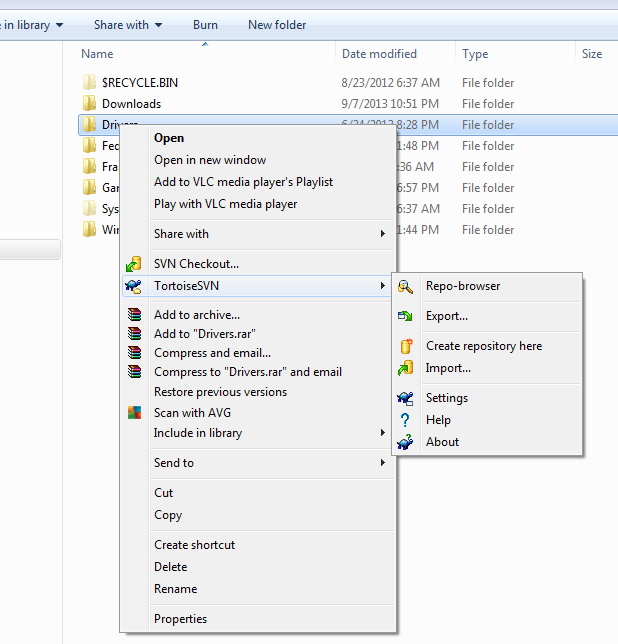
\includegraphics[scale=0.75]{TortoiseSVNContextMenu.png}
\caption{TortoiseSVN context menu}
\label{TortoiseSVN-context-menu}
\end{figure}
\section{Creating a Repository}
A repository can be any folder located anywhere on a computer that is supposed to be accessible by team members. You can also make a repository on your computer just for testing purposes. Remember, you never make changes to the repository directly. You create a local copy and then use subversion tool to commit changes. Several websites offer free space to host subversion repositories, for example, GoogleCode (\url{code.google.com}).
\begin{figure}[H]
\centering
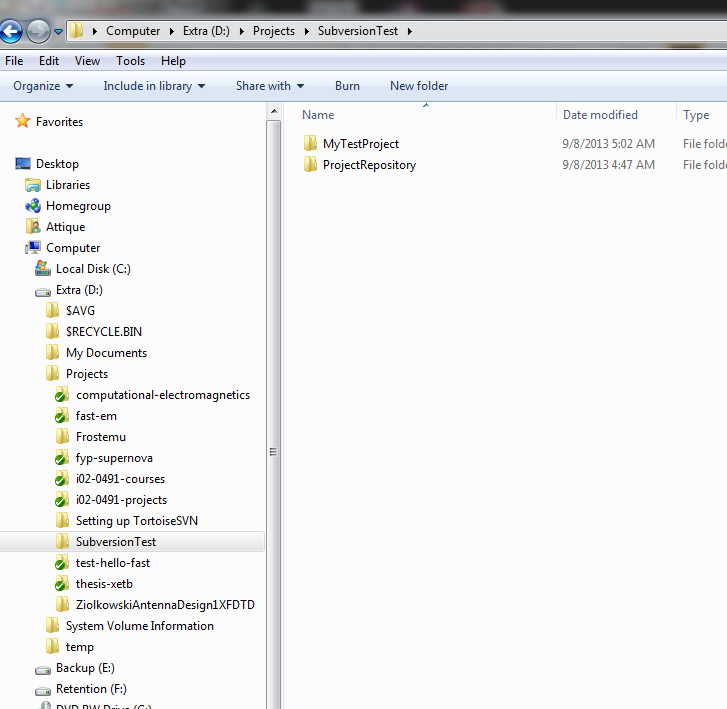
\includegraphics[scale=0.75]{RepositoryandProjectFolders.png}
\caption{Creating repository and project folders.}
\label{Repository-and-project-folders}
\end{figure}
Creating a repository is simple. Pick any empty folder, open up right--click menu, go into TortoiseSVN sub--menu and click `Create repository here' (figure \ref{Creating-subversion-repository}). Now we need to checkout a local copy of the repository in which we'll be doing all our work. Right--click on the project folder and select `SVN Checkout...' (figure \ref{SVNCheckout}). Enter the URL of the repository (figure \ref{Checkout-URL}). Also select checkout depth as `Immediate children, including folders'. Since we've already created a folder we don't want fully recursive checkout. When checking out your online repository on GoogleCode, you'll select `fully recursive'. If checkout is successful you'll get a dialog box as shown in figure \ref{Checkout-finished}. There will also be a green icon on the project folder indicating everything is updated and no changes have been made to the local copy.

All commits to the repository are tracked and have a revision number. Revision number is the smallest unit of a program version number. Everytime changes are committed revision number increases by one. The project can be \textit{reverted} back to any revision. Any changes from a particular revision can also be reverted.
\begin{figure}[H]
\centering
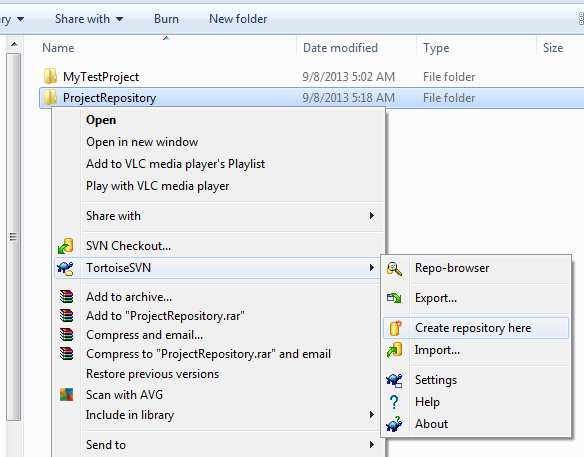
\includegraphics[scale=0.75]{CreatingaRepository.png}
\caption{Creating a subversion repository.}
\label{Creating-subversion-repository}
\end{figure}
\begin{figure}[H]
\centering
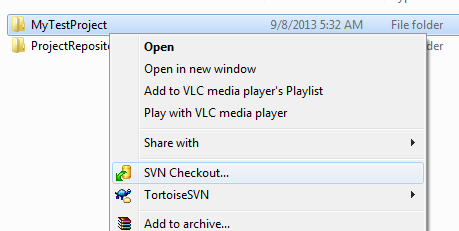
\includegraphics[scale=0.75]{SVNCheckout.png}
\caption{SVN Checkout.}
\label{SVNCheckout}
\end{figure}
\begin{figure}[H]
\centering
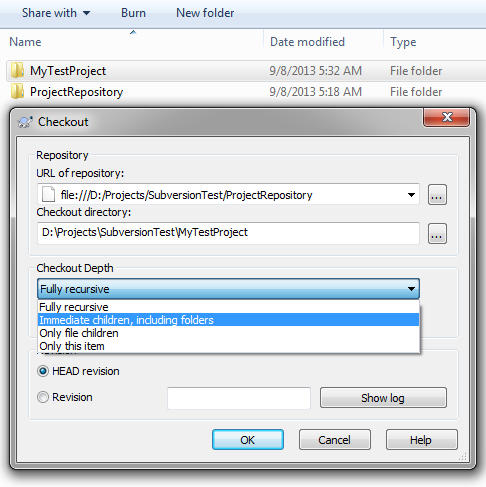
\includegraphics[scale=0.75]{CheckoutandRepositoryURL.png}
\caption{Repository URL.}
\label{Checkout-URL}
\end{figure}
\begin{figure}[H]
\centering
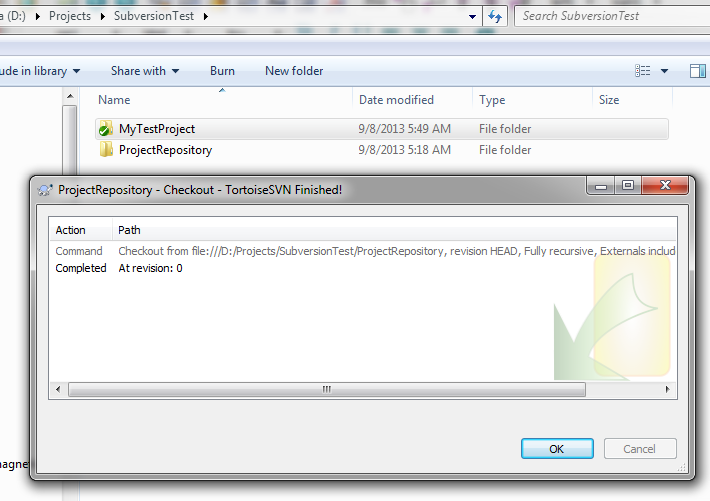
\includegraphics[scale=0.75]{CheckoutFinished.png}
\caption{Successful checkout.}
\label{Checkout-finished}
\end{figure}
\section{Adding New Files to the Project}
Now we want to make a hello world project using Visual Studio 2010. This is an empty win32 console application as shown in figure \ref{VS2010-new-project}. We'll write a hello world program and add the relevant files to our subversion project.

Newly created files are referred to as `unversioned'. Versioned files have a defined role. Unversioned files or folders have a blue question mark icon shown in figure \ref{unversioned-files}.

We're only going to add the essential files and ignore temporary files or any files that are created as a result of compilation. Select all the files that are to be added and add them using the TortoiseSVN menu (figure \ref{adding-files}). Newly added files that are not committed yet have a blue plus icon. Next we're going to ignore all the non--essential files/folders (figure \ref{ignoring-files}). These will be not be tracked for changes.

One way to figure out which files to ignore is to ask yourself, ``Can I delete these files (to save space) without affecting anything?'' The ignored files and folders in this case are created when the project is compiled. You may already know that `debug' folder contains the exe file and any temporary files created during the $pre-process > compile > assemble > link$ cycle. You can safely delete this folder because it is created every time the program is compiled. 
\begin{figure}[H]
\centering
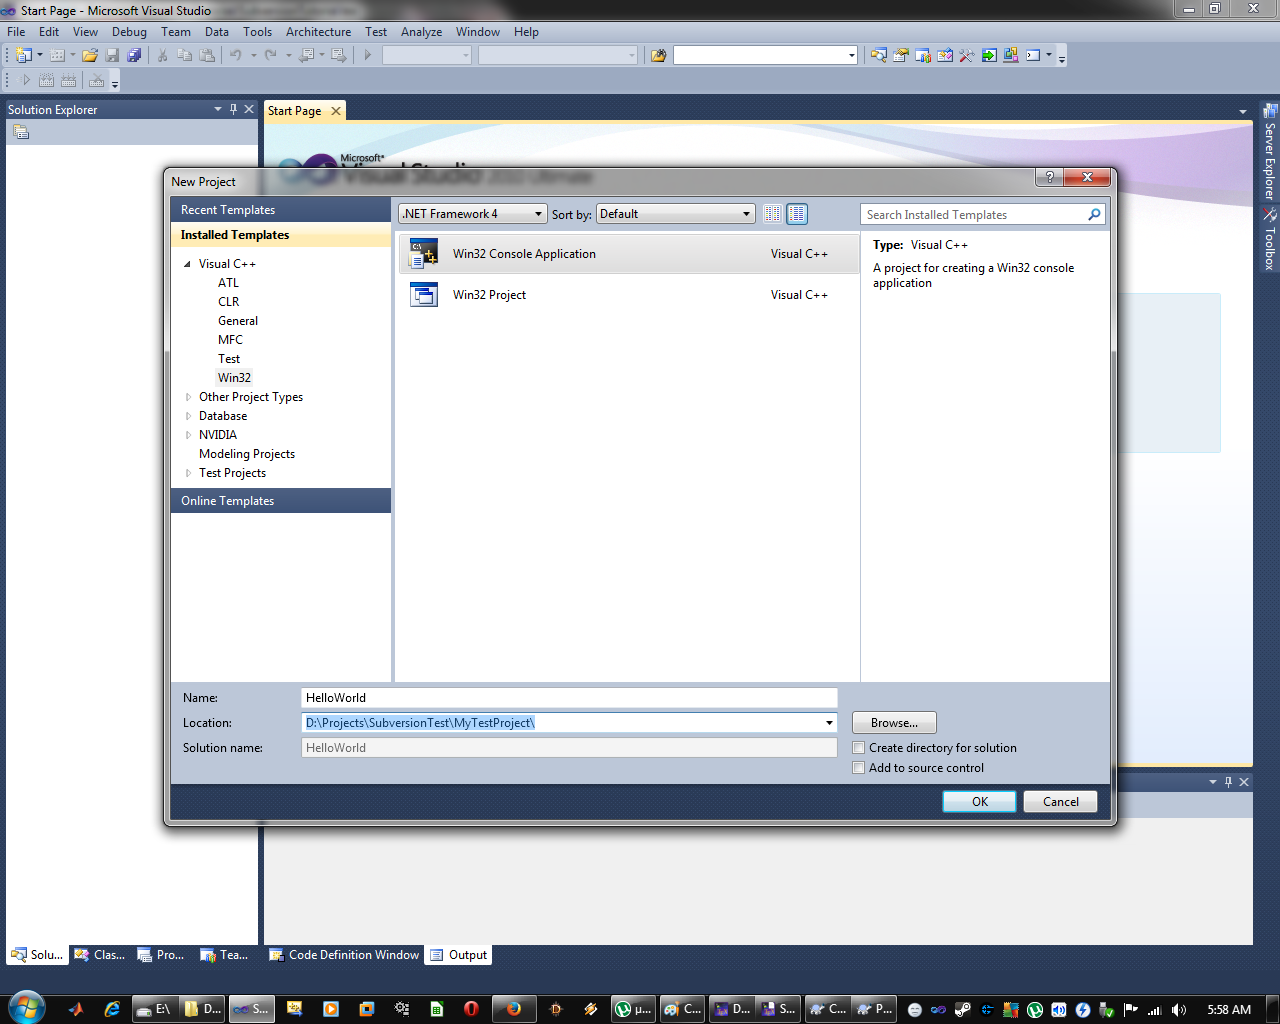
\includegraphics[scale=0.45]{NewProjectinVS2010.png}
\caption{Creating an empty project in Visual Studio 2010.}
\label{VS2010-new-project}
\end{figure}
\begin{figure}[H]
\centering
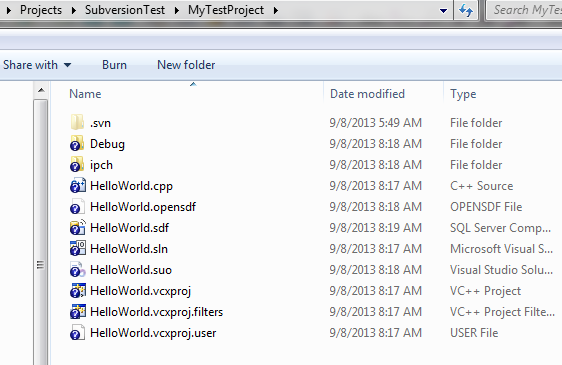
\includegraphics[scale=0.75]{UnversionedFiles.png}
\caption{Unversioned files.}
\label{unversioned-files}
\end{figure}
\begin{figure}[H]
\centering
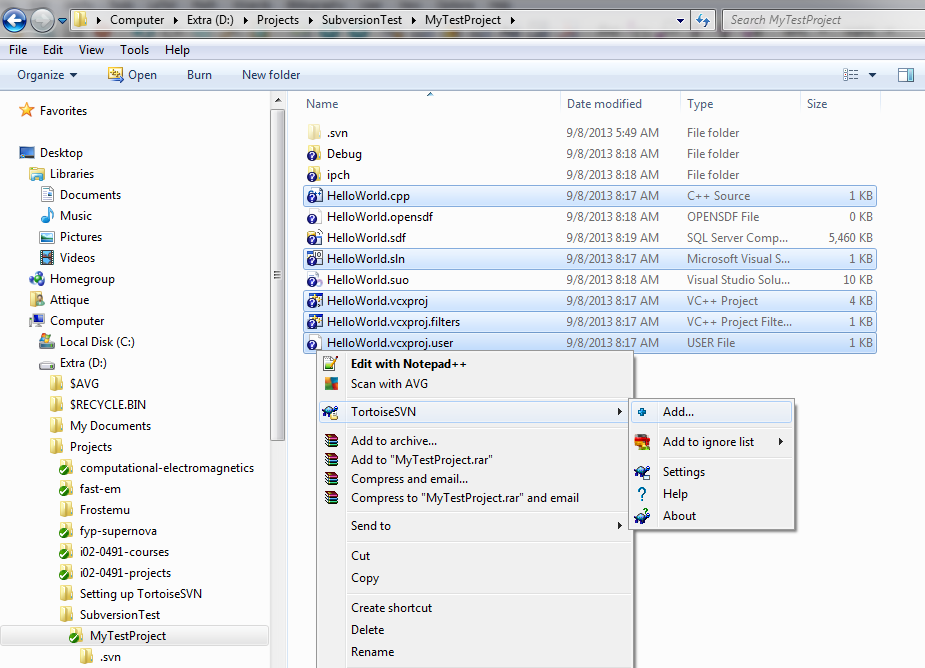
\includegraphics[scale=0.7]{AddingFiles.png}
\caption{Adding files.}
\label{adding-files}
\end{figure}
\begin{figure}[H]
\centering
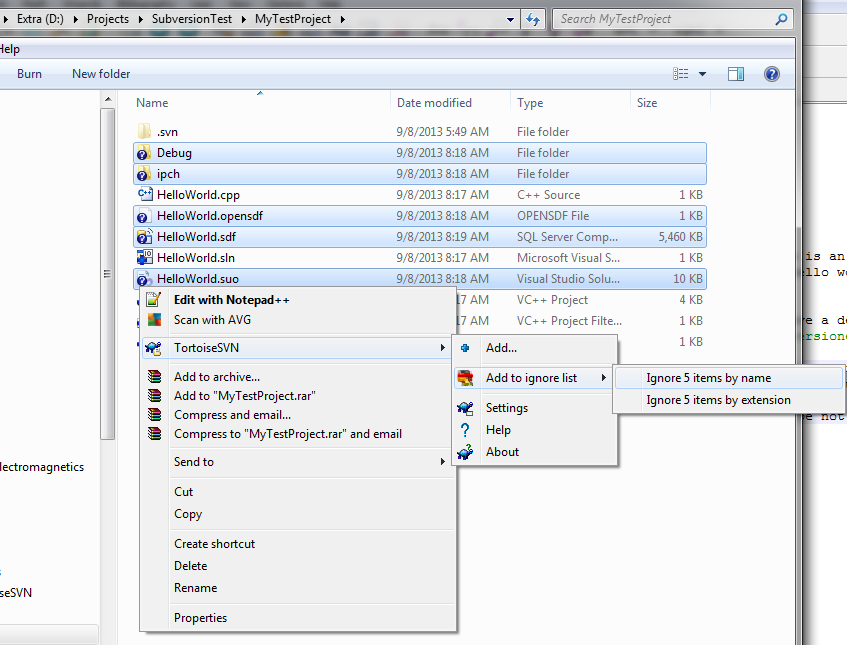
\includegraphics[scale=0.7]{IgnoringFiles.png}
\caption{Adding items to ignore list.}
\label{ignoring-files}
\end{figure}
\section{Committing Changes}
Before committing our code is as shown in figure \ref{code-before-committing}. The files in project folder look as shown in figure \ref{project-before-committing}. Also note that project folder has a red icon indicating we've made changes to it and have not committed them to the repository yet.

To commit the changes, right--click the project folder and select `Commit'. You'll have enter a message detailing a list of changes you made (figure ). This message is added to a log known as the `changelog'.

Everytime a group member commits changes to the repository other group members in the project must update their local copies to remain up--to--date.
\begin{figure}[H]
\centering
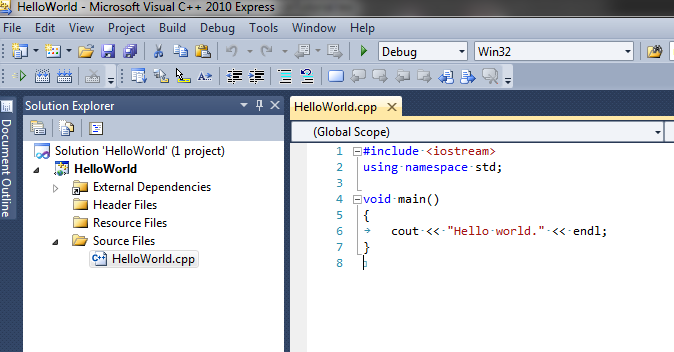
\includegraphics[scale=0.75]{ProgramBeforeCommit.png}
\caption{Program code before committing.}
\label{code-before-committing}
\end{figure}
\begin{figure}[H]
\centering
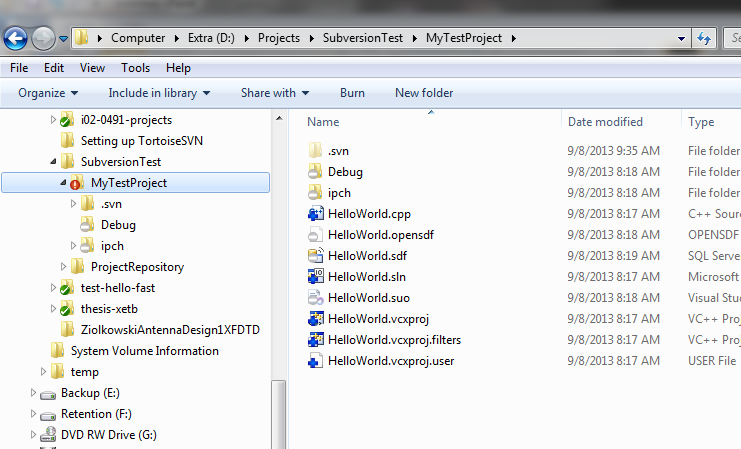
\includegraphics[scale=0.75]{ProjectBeforeCommit.png}
\caption{Project folder and files before committing.}
\label{project-before-committing}
\end{figure}
\begin{figure}[H]
\centering
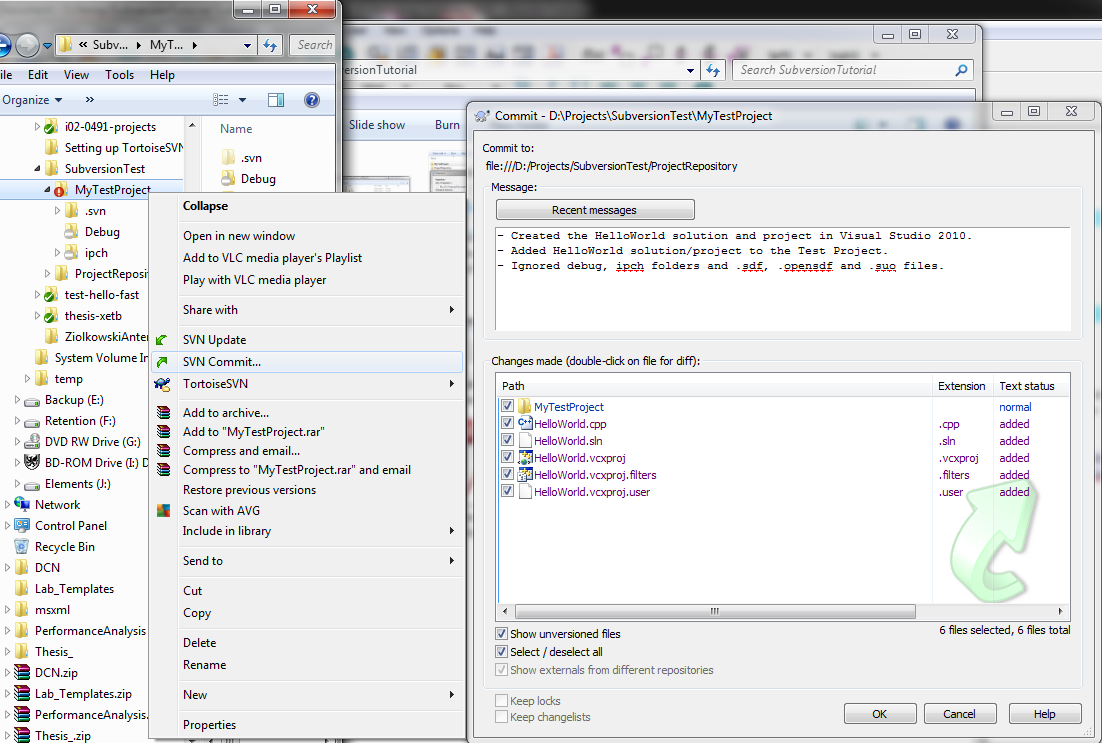
\includegraphics[scale=0.50]{CommitMessage.png}
\caption{Committing changes.}
\label{commit-message}
\end{figure}
\section{Using the Changelog}
Suppose someone in the group decides that they should be using standard C++ conventions and objects at main() not returning a value. They change the code to reflect this as shown in figure \ref{Main-changed}. All the revisions and commits can be inspected using the changelog option. To view changelog right--click the project folder and select `Show Log' from the TortoiseSVN sub--menu as shown in figure \ref{show-log}.

The changelog window shows a list of all the latest revisions in the upper window (figure \ref{changelog}). By selecting a revision, a list of files and description of changes will appear in the lower window. To view what exactly was changed in a particular file, right--click the filename from the lower window and select `Show Changes'. A program called `Diff Viewer' will open and open old and modified versions of the file side--by--side highlighting the changes as shown in figure \ref{diff}.

Needless to say, changelog is the most effective means of communication between group members in a large project. Everybody can easily see what going on, exactly which files are being modified, what are the modifications and by whom.
\begin{figure}[H]
\centering
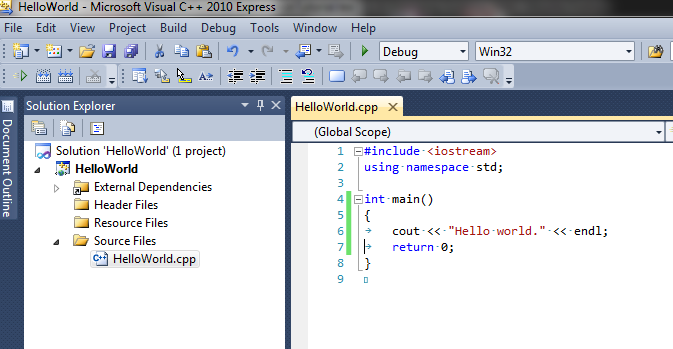
\includegraphics[scale=0.75]{MainChanged.png}
\caption{Changes to code.}
\label{Main-changed}
\end{figure}
\begin{figure}[H]
\centering
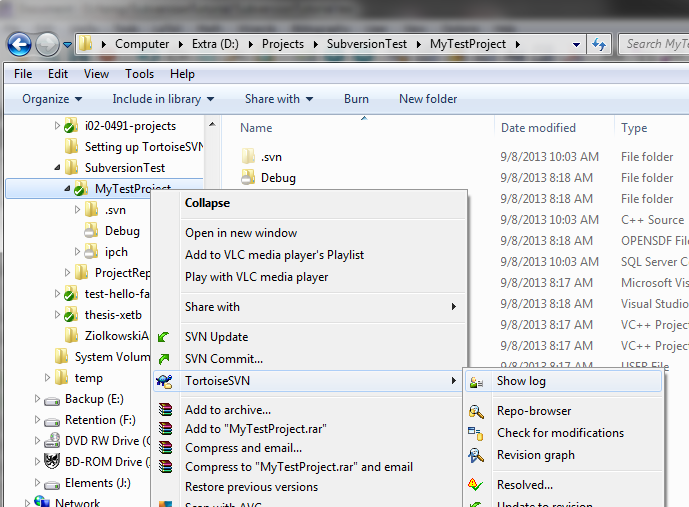
\includegraphics[scale=0.75]{ShowLog.png}
\caption{Accessing changelog.}
\label{show-log}
\end{figure}
\begin{figure}[H]
\centering
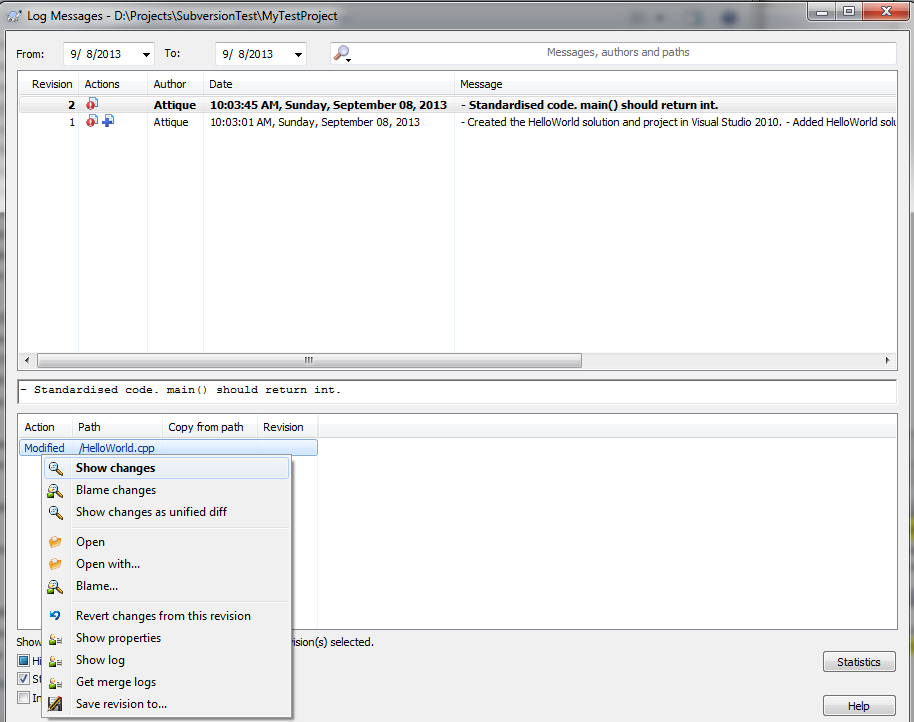
\includegraphics[scale=0.65]{ChangeLog.png}
\caption{The changelog.}
\label{changelog}
\end{figure}
\begin{figure}[H]
\centering
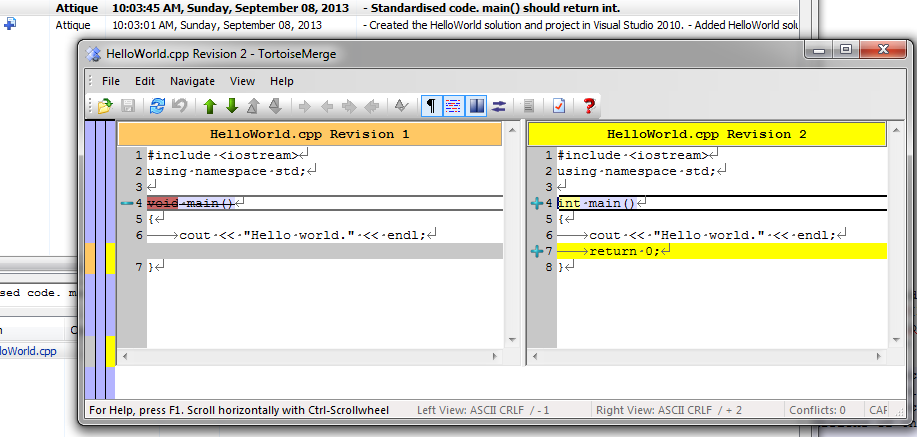
\includegraphics[scale=0.65]{DiffViewer.png}
\caption{The diff of old and modified files.}
\label{diff}
\end{figure}
\section{Reverting Changes}
If someone in the group doesn't like the changes made in revision 2 they can go back to revision 1 from the changelog. By selecting `Revert to this Revision' from the right--click menu the project will be effectively rolled back to where it was before revision 2 (figure \ref{reverting}).
\begin{figure}[H]
\centering
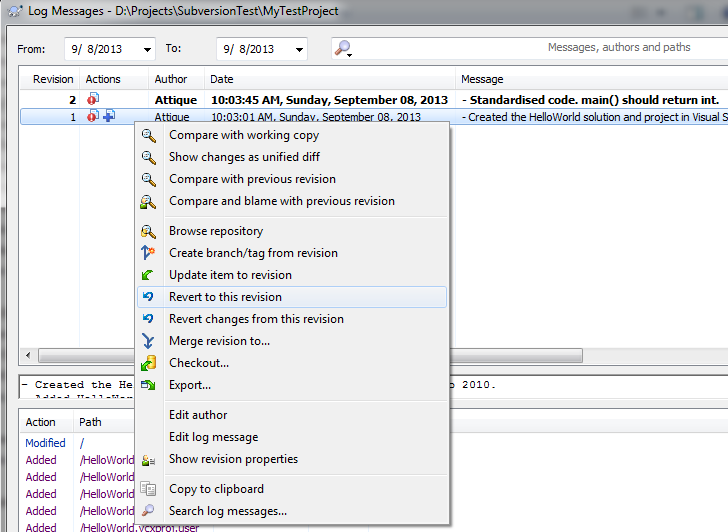
\includegraphics[scale=0.65]{Reverting.png}
\caption{Reverting or rolling back to an earlier revision.}
\label{reverting}
\end{figure}
%\nocite{*}
\bibliographystyle{plain}
\bibliography{PhysicsRef}
\end{document}
